\documentclass{standalone}
% 公式
\usepackage{amsmath}
% 公式符号加粗
\usepackage{bm}
% TikZ 图形
\usepackage{tikz}
% 插入三维图形
\usepackage{pgfplots}
\pgfplotsset{width=7cm,compat=1.18}
% colorbrewer 系列调色板 PuBu-9
\usetikzlibrary{pgfplots.colorbrewer}

\begin{document}
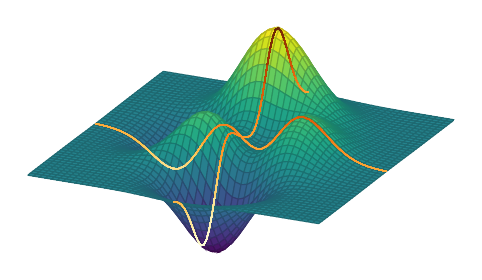
\begin{tikzpicture}
\begin{axis}[
    hide axis,
    colormap/viridis,
]
\addplot3[
    surf,
    samples=50,
    domain=-3:3,
]
{3*(1-x)^2*exp(-x^2 - (y+1)^2) - 10*(x/5 - x^3 -y^5)*exp(-x^2 -y^2) - 1/3*exp(-(x+1)^2 -y^2};

\addplot3[
   variable=t,
   mesh,
   samples=50,
   colormap/YlOrBr,
   domain=-3:3
] (0, t, {3*exp(- (t+1)^2) - 10*(-t^5)*exp(-t^2) - 1/3*exp(-1 -t^2});

\addplot3[
   variable=t,
   mesh,
   samples=50,
   colormap/YlOrBr,
   domain=-3:3
] (t, 0, {3*(1-t)^2*exp(-t^2 - 1) - 10*(t/5 - t^3)*exp(-t^2) - 1/3*exp(-(t+1)^2});

\end{axis}
\end{tikzpicture}
\end{document}
